\chapter{Evaluierung der erstellten Modelle} % (fold)
\label{cha:eval_modell}

\section{Hypothesen} % (fold)
\label{sec:m_hypothesen}

\subsection{Konzeptuell begründete Hypothesen} % (fold)
\label{sub:m_konzeptuell_begründete_hypothesen}

\begin{hyp}
	Das Werkzeug schränkt Benutzer nicht bei der Externalisierung ihrer mentalen Modelle ein.
\end{hyp}
Offenheit, Anzahl der Element-Arten
	
\begin{hyp}
	Das Werkzeug ermöglicht die Repräsentation beliebig komplexer Modelle.
\end{hyp}
Größe der Oberfläche, Einbettungen

\begin{hyp}
	Das Werkzeug ermöglicht die Abstimmung individuelle Modelle.
\end{hyp}
kollaborative Modellbildung

% subsection konzeptuell_begründete_hypothesen (end)

\subsection{Explorativ gebildete Hypothesen} % (fold)
\label{sub:m_explorativ_gebildete_hypothesen}

\begin{hyp}
	Zur Abbildung von Zusammenhängen ist die Verwendung von Verbindern nicht notwendig.
\end{hyp}
Connectedness

% subsection explorativ_gebildete_hypothesen (end)

% section hypothesen (end)

\section{Untersuchungsdesign und Durchführung} % (fold)
\label{sec:m_untersuchungsdesign}

% section untersuchungsdesign (end)

\section{Ergebnisse} % (fold)
\label{sec:m_ergebnisse}

% section ergebnisse (end)

\subsection{Connectedness} % (fold)
\label{sub:connectedness}

\begin{figure}[htbp]
	\centering
		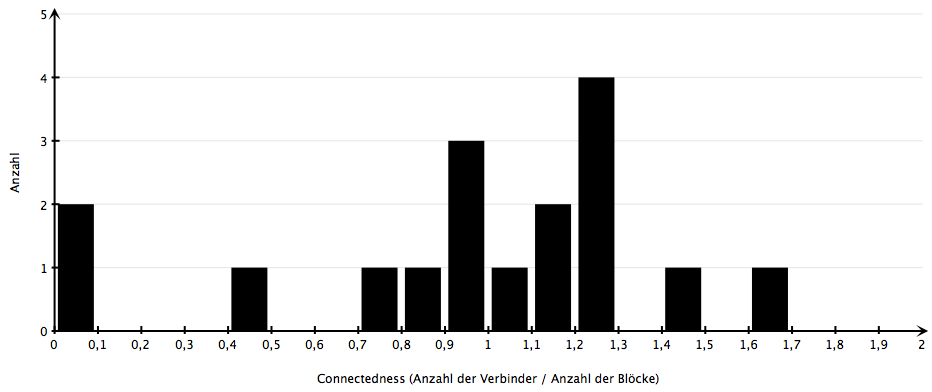
\includegraphics[width=12cm]{img/Evaluierung/connectednessConceptMapping.png}
	\caption{Connectedness -- Concept Mapping}
	\label{fig:img_Evaluierung_connectednessConceptMapping}
\end{figure}

\begin{figure}[htbp]
	\centering
		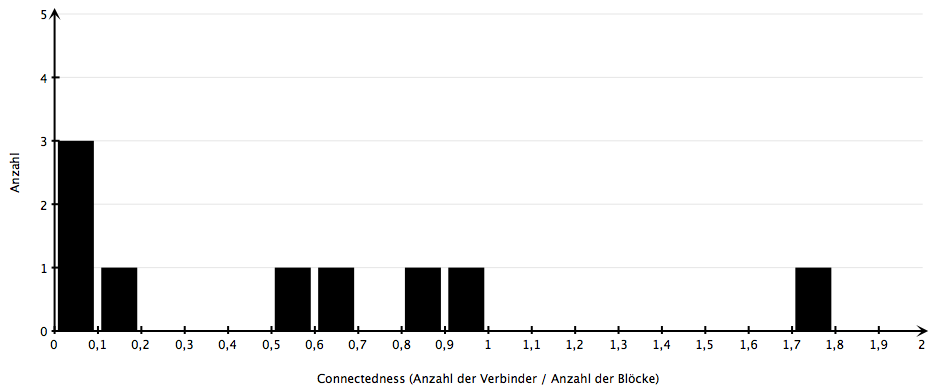
\includegraphics[width=12cm]{img/Evaluierung/connectednessAushandlung1.png}
	\caption{Connectedness -- Aushandlung (1. Durchgang)}
	\label{fig:img_Evaluierung_connectednessAushandlung1}
\end{figure}

\begin{figure}[htbp]
	\centering
		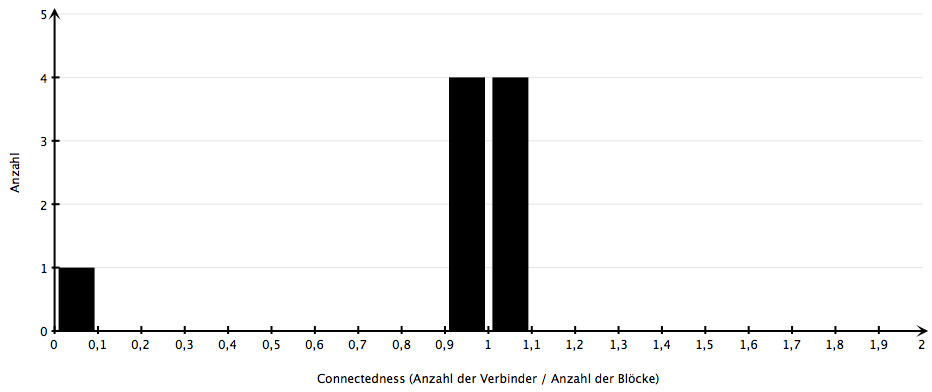
\includegraphics[width=12cm]{img/Evaluierung/connectednessAushandlung2.png}
	\caption{Connectedness -- Aushandlung (2. Durchgang)}
	\label{fig:img_Evaluierung_connectednessAushandlung2}
\end{figure}

% subsection connectedness (end)

% chapter eval_modell (end)